\pagestyle{empty}
\cleardoublepage
\pagestyle{fancy}
\chapter{Conclusão e trabalhos futuros}\label{cap4}

Este trabalho apresentou um estudo na área de decomposição de domínio para a geração de malhas em paralelo. Já foi dado início ao desenvolvimento de uma técnica bidimensional de geração de malha baseada numa decomposição utilizando \textit{quadtree}.

O trabalho proposto pode ser dividido basicamente em duas etapas. A primeira consiste em receber a entrada e dividi-la em partes que possam ser tratadas novos domínios independentes. Todos essas partes, por sua vez, possuem a quantidade de carga aproximadamente equivalentes.

A técnica proposta utiliza uma \textit{quadtree} para estimar a carga de cada subdomínio que for gerado para se obter um bom balanceamento de carga entre os processadores.

A segunda etapa é a geração da malha em cada um dos novos domínios. Qualquer algoritmo de triangulação dado uma borda como entrada pode ser utilizado, podendo, inclusive, serem empregados algoritmos diferentes nos subdomínios. Além da triangulação, é necessário fazer a junção das diversas malhas geradas em uma só.

Para esse trabalho estou propondo uma técnica de geração de malha por avanço de fronteira por particionamento do domínio em paralelo. O foco da técnica é a subdivisão dos domínios e não a geração da malha. Apesar de qualquer algoritmo poder ser utlizado, em particular, o algoritmo de avanço de fronteira que estou utilizando para gerar malha está em \cite{bib:Miranda99} e \cite{bib:Cavalcante-Neto01}.

\section{Cronograma}
O cronograma de estudos e trabalho para conclusão da dissertação de mestrado pode ser visto na Figura~\ref{fig:tabela}.

 \begin{figure}[htbp]
     \begin{center}
     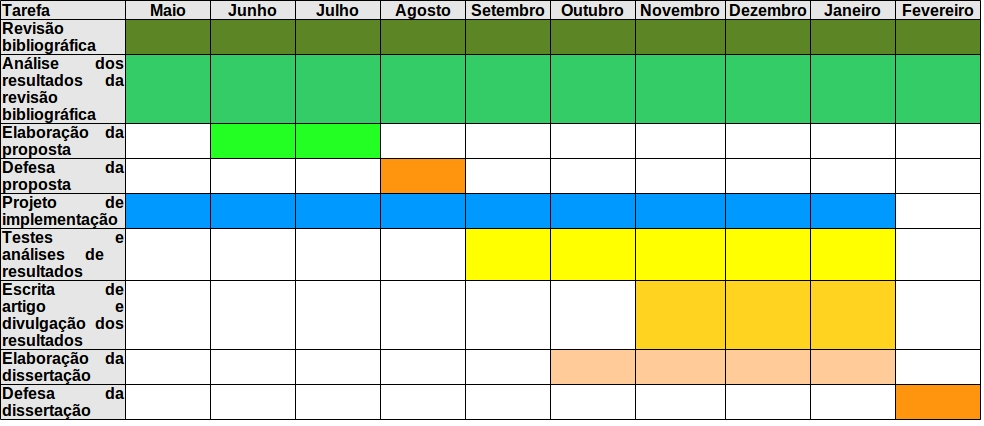
\includegraphics[width=1.1\textwidth]{tabela}
     \caption{Cronograma de estudos e trabalho para conclusão da dissertação de mestrado.} 
     \label{fig:tabela}
     \end{center}
 \end{figure}